\documentclass[letterpaper,10pt]{article}

\usepackage[english]{babel}
\usepackage[utf8]{inputenc}
\usepackage{amsmath}
\usepackage{graphicx}
\usepackage[colorinlistoftodos]{todonotes}
\usepackage[top=1in, bottom=1in, left=1in, right=1in]{geometry}
\usepackage[small]{titlesec}

\newcommand{\bes}{\begin{equation*}}
\newcommand{\ben}[1]{\begin{equation}\label{#1}}
\newcommand{\ees}{\end{equation*}}
\newcommand{\be}{\begin{equation}}
\newcommand{\ee}{\end{equation}}

\newcommand{\vkl}{v_{k,\ell}}
\newcommand{\vklm}{v_{k,\ell-1}}
\newcommand{\vklp}{v_{k,\ell+1}}
\newcommand{\vkml}{v_{k-1,\ell}}
\newcommand{\vkpl}{v_{k+1,\ell}}
\newcommand{\vkmlp}{v_{k-1,\ell+1}}
\newcommand{\vkplp}{v_{k+1,\ell+1}}

\begin{document}

\begin{flushright}
{\Large Josh Bevan - HW1 Q2 - CS555}
\end{flushright}
\vskip -0.1in
\hrule
\vskip 0.3in

\hskip -.3in{\large \textit{For $x \in [0,1]$ and $u_t + u_x = 0$, consider two ICs: square wave and Gaussian. For each of these cases, implement the forward upwind scheme. Use periodic boundary conditions.}

\section*{Establish numerically the rate of convergence using a discrete $L^2$-norm.}
Fixed $\lambda = 0.8$ was chosen so that integer number of time steps needed for 1 time period.
\begin{figure}[!htb]
\centering
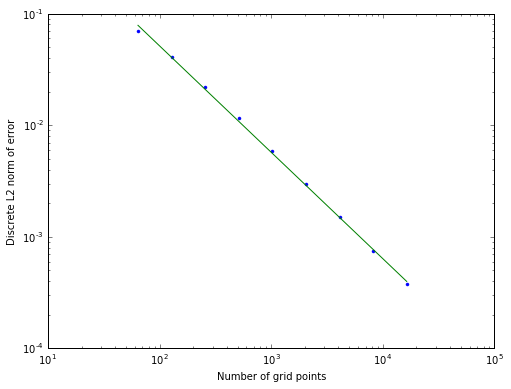
\includegraphics[width=0.6\textwidth]{ga.PNG}
\caption{Rate of convergence of Gaussian initial condition, rate of convergence from linear fit: 0.953}
\end{figure}

\begin{figure}[!htb]
\centering
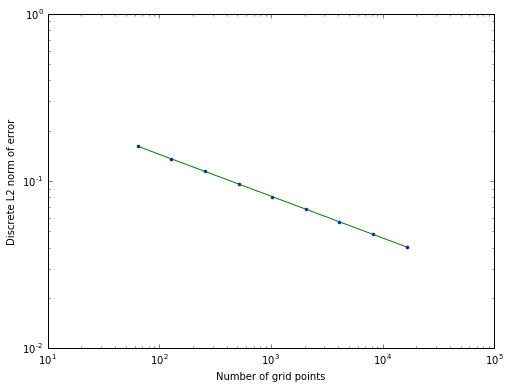
\includegraphics[width=0.6\textwidth]{sq.PNG}
\caption{Rate of convergence of square wave initial condition, rate of convergence from linear fit: 0.249}
\end{figure}

\section*{Please comment on why a fixed $\lambda$ is useful here.}
A consistent, stable scheme converges as $\Delta x, \Delta t \rightarrow 0$. To assess convergence properties then, both the mesh spacing and the time interval needs to be decreased. It is a good idea to decrease both of these by the same proportion for each run, so that all runs are directly comparable to each other. If we wish to decrease both by the same proportion each run, then the result is a constant $\lambda$.

\section*{Is the scheme convergent? Do you observe a different order of convergence depending on the initial condition function? Discuss.}
The scheme is convergent; as both the time interval and mesh spacing is decreased the norm of the error between the numerical and exact solutions continues to decrease.

In the Gaussian IC, the order of convergence is very nearly 1st order, which is to be expected given the first order terms dominate the truncation error. However, in the square wave test case an order of convergence of only ~0.25 was observed. One can explain this from two different avenues: First, from a numerical standpoint the truncation error terms depend on the derivatives of the solution. The discontinuity in the square wave means that there are exceptionally high derivatives at the discontinuities, leading to large truncation errors locally. Second, intuitively one can observe the spatial/temporal evolution of the square wave and note that in smooth regions (far from the discontinuity) the local error is quite good. Near the discontinuity numerical diffusion smears the square wave leading to localized, but high, errors. Increasing refinement for the square wave reduces the width of the discontinuity smear, but the amplitude of the absolute error at the discontinuity remains quite high even for comparatively small mesh spacing. The result is that while refinement does reduce the norm of the error, it doesn't work as well as one may expect at reducing the error \textit{everywhere} in the domain.

\end{document}

%\begin{figure}[!htb]
%\centering
%\includegraphics[width=0.6\textwidth]{Unrolled.PNG}
%\caption{\label{fig:unrolled}"Unrolled" ring, coincident nodes at either end.}
%\end{figure}